\chapter{Tandem mass spectrometry for protein analysis}\label{chap:msms}

% TODO To následující by bylo možná dobré intro, nějak prožezané do pár odstavců.

Proteins are amino acid biopolymers that take part in most natural processes in living organisms. Among other things, they are vital for cell growth, reproduction, metabolism, and movement. [citace] Proteins are also a frequent target of medicine, because they play a key role in most diseases [citace nějakého proteinového léku].

Protein function is highly dependent on its 3D structure [citace], and as was shown by Anfinsen [citace], the information about the structure is in turn encoded in the sequence of the protein.

Protein folding is driven by natural biophysical forces which makes it hard to properly recreate \emph{in silico}, especially when there is no homologous protein with known structure [citace]; this problem is called \emph{de novo} folding.

Techniques for \emph{de novo} folding rely mostly on molecular dynamic simulations. These approaches are often very performance-intensive (?), because they are effectively optimising a complicated scoring function a huge multidimensional problem space. [citace] Any information we have about the structure can be thus very heplful in reducing the problem space when supplied to the algorithm, making the computations faster and more accurate. One type of such information are the positions of disulphide bridges.

Disulphide bridges (DB) in proteins can be formed between the sulfhydryl groups of two cysteines during a thiol–disulfide exchange reaction catalyzed by thioredoxin [citace] In vivo they are oftentimes essential to correct protein folding, because they stabilise the final structure [citace] The knowledge of DB positions can be used, among other things, to constrain the molecular dynamic simulations, as mentioned earlier. In addition, the knowledge of which cysteines do \emph{not} partake in a DB is important, too.

Non-interlinked cysteines have an important pH-regulating function within proteins [citace] (a něco dalšího ještě?). Consequently, cysteines are scarce compared to other amino acids [citace], but they are usually very well conserved during evolution [citace].

There are many methods aiming to determine the positions of DBs, on of them is tandem mass spectrometry combined with liquid chromatography (LC-MSMS). LC-MSMS is a popular general analysis technique, often used in proteomics for its accuracy and relative straightforwardness of the experiments (?) [citace].

In LC-MSMS, the protein is eventually fragmented to smaller charged peptides whose mass to charge ratio (\(m/z\)) is measured with atomic precision. The whole experiment can be designed in a way that the DBs are preserved which results in the occurence of \emph{breptides} with specific \(m/z\) fragmentation signatures. Computational analysis can help us discover these fragmentation spectra and determine the original positions of the DBs in the protein.

% TODO ... a tohle jsme si dali za task; deteminovat pozici DBs z hmotnostních spekter.

% TODO Bridgetid je interlikend peptide, s 2+ segmenty.

% TODO V následujících několika sekcích si vysvětlíme principy hmotností spektrometrie, s focusem na přístupy a poznatky, které jsou relevantní pro naši práci. Kde to je možné, tam se odvoláváme na common přístupy a srovnáváme je s našimi konrétními potřebovami v kontextu tohoto tasku. Na konci této kapitoly formulujeme na základě této teorie formulujeme konkrétní problém a jeho přibližnou komplexitu.


\section{Sample preparation}

% TODO Ještě před MS je nutné připravit vzorek tak, aby s ní vůbec fungoval.

To prepare the protein for the analasis, it needs to be proteolyticaly cleaved; trypsin, and, to a lesser extent, pepsin, are popular choices. Trypsin is a serine protease with very high specificity which makes it very useful for mass spectrometry analyses, because the resulting peptides are predictable.

Trypsin cleaves amino acid chains at the carboxyllic side of lysine and arginine, provided they are not followed by proline~\cite{olsen2004trypsin}. Lysine and arginine are both relatively abundant in most proteins which makes the tryptic digestion peptides --- or as we will call them, \emph{tryptides} --- reasonably sized for a mass spectrometry analysis~\cite{matthiesen2020trypticsize}. With that being said, the sample protein is not cleaved at every potential cleavage place; so called \emph{missed cleavages} do occur, and their frequency and position depend on neigbouring residues~\cite{gershon2014cleaved}, and experimental setup.

% TODO Trypsin je sice populární, bylo nicméně ukázáno že je aktivní při pH, které nědky způsobuje scrambling můstků [citace]. Tento jeho efekt je složité omezit, protože při nižším pH špatně štěpí [citace]. Někdy se proto ppoužívají jiné proteázy, například pepsin nebo [doplnit] [citace]. Pepsin je však zase méně specifický, takže když nemáme tight controlu nad digestion, vznikají nám příliš malé fragmenty, které je někdy složité detekovat[citace]. Jak přesně pepsin kontrolovat se často liší vzorek od vzorku [citace].

% TODO vzorky se v rámci sample preparation často redukují a alkylují, aby se přerušily DBs, které komplikují fingerpriting a prohledávání databází [citace na nějaký normální proteomický experiment]. Naším cílem je však interlinkované bridgetidy identifikovat, takže tento krok v našem hlavním vzorku přesakujeme.

After digestion, the resulting peptides undergo separation in liquid chromatography.

\section{Sample separation}

In a general proteomic experiment, the signal from more abundant sample proteins may interfere with the other, less frequent proteins. To sidestep this problem, it has become routine to perform separation before the main MS experiment, separating the sample either on the protein level or the peptide level.

One possible method for protein-level separation is two dimensional polyacrylamide gel electrophoresis, during which the proteins are split first by isoelectric focusing, and then by SDS gel electrophoresis~\cite{o1975high}. 2D-PAGE has very high resolution~\cite{klose1995two}. The proteins are usually digested in-gel after the separation, manually cut out, and then put into the mass spectrometer, causing the method to have relatively low throughput~\cite{patton2002two}, making it unfit for some scenarios.

In our scenario with one protein per sample, separating on protein-level is not going to be useful; instead, peptide-level separation is preferred. A popular peptide-level separation method is liquid chromatography (LC). In a model MS-based proteomic LC experiment, the proteins are digested without prior separation, and the resulting peptides are separated on reverse-phase liquid chromatography column that is directly connected to a tandem mass spectrometer~\cite{washburn2001large}. Usually the number of different proteins in the sample is high, leading to a large amount of generated spectra and causing a need for automatic processing. This type of identifying sample proteins is sometimes called shotgun processing.

Reverse-phase LC has two main constituents: a mobile liquid phase containing the peptides and a stationary solid phase which is usually a nonpolar column with \(\ce{C18}\) alkyl chains~\cite{chang1976high}. The mobile phase passes along the stationary phase, the elution time of each individual peptide depending on its hydrophobic interactions with the alkyls. The peptides are eluted with a polar mixture of water and organic solvent, such as acetonitrile~\cite{frohlich2006proteome}, the shortest and least hydrophilic eluting the earliest.


\section{Tandem mass spectrometry}

Mass spectrometry is an analytical technique with roots deep in the last century that has originally been used for studying small thermostable molecules. However, with the advancements in soft ionization allowing proteins and other biomolecules to be analysed as well~\cite{fenn1989electrospray}, mass spectrometry has become an indispesable tool in proteomics research~\cite{collins2003human}.

In the context of proteomics, mass spectrometry experiments can be either single-stage or tandem. During single-stage experiments, the mass distribution of a polypeptide sample is determined. The more frequent of the two, tandem (MS/MS) mass spectrometry is used to learn about certain structural features of a protein, including sequence and post-translational modifications.

\begin{figure}
  \centering
  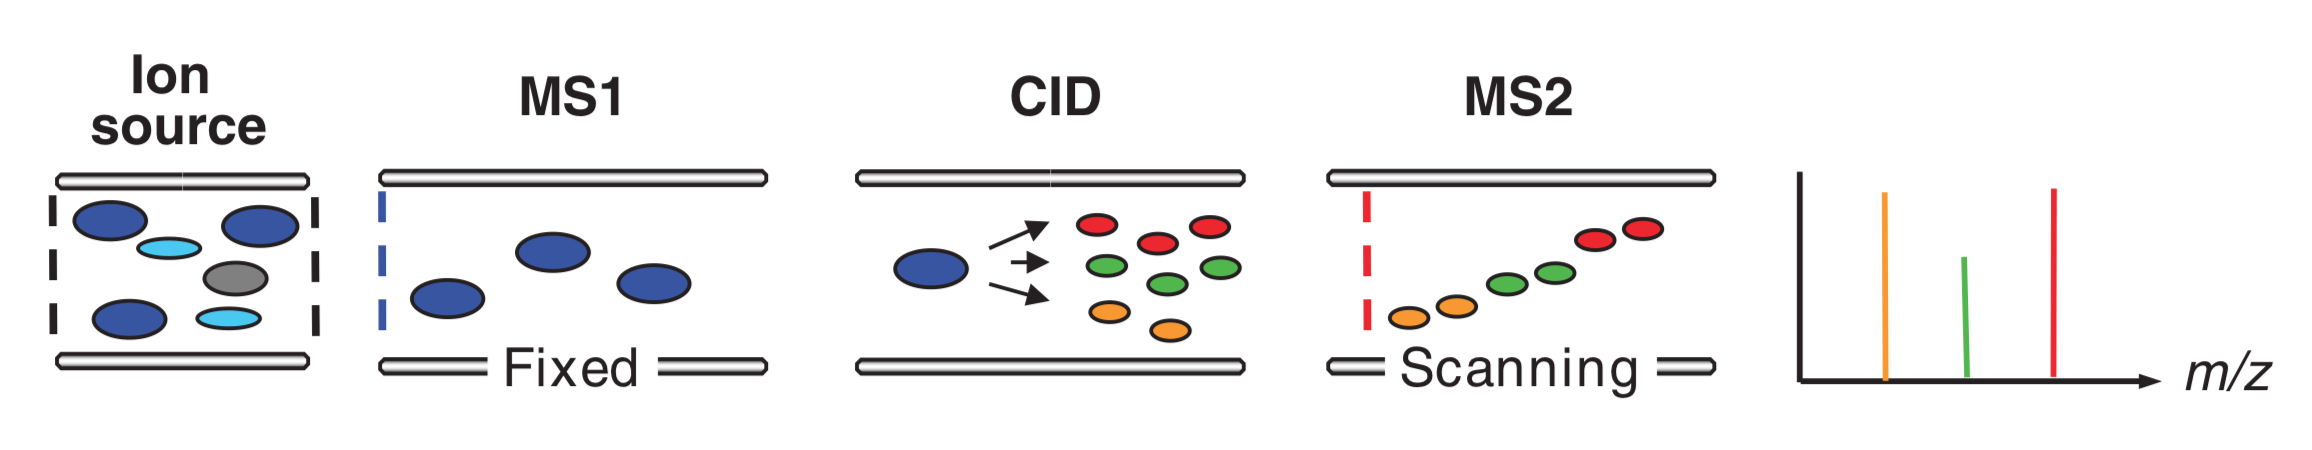
\includegraphics[width=.9\linewidth]{img/msms-workflow.png}
  \caption{An ordinary MS/MS workflow diagram. While the specific intrumentation details differ from spectrometer to spectrometer, the general structure of ionize \textrightarrow{} analyse \textrightarrow{} fragment \textrightarrow{} analyse is common to all of the MS/MS spectrometry experiments. Image taken from~\citet{domon2006mass}.}\label{fig:mass-spectrometry-workflow}
\end{figure}

Both the single-stage and MS/MS experiments begin similarly: the sample peptides are ionized, the ions travel through an electromagnetic field in an analyser and into a detector, whilst their mass-to-charge (\(m/z\)) is being calculated~\cite{gross2006mass}. In single-stage mass spectrometry, the experiment ends there, while in MS/MS, some of these \emph{precursors} are selected to undergo fragmentation in the collision cell, as shown in \Cref{fig:mass-spectrometry-workflow}. The resulting fragments are also analysed and their \(m/z\) values noted; the output of the MS/MS experiment are the precursor masses and their fragmentation spectra, an example of which can be seen one figure \Cref{fig:frag-spectrum}.

\begin{figure}
  \centering
  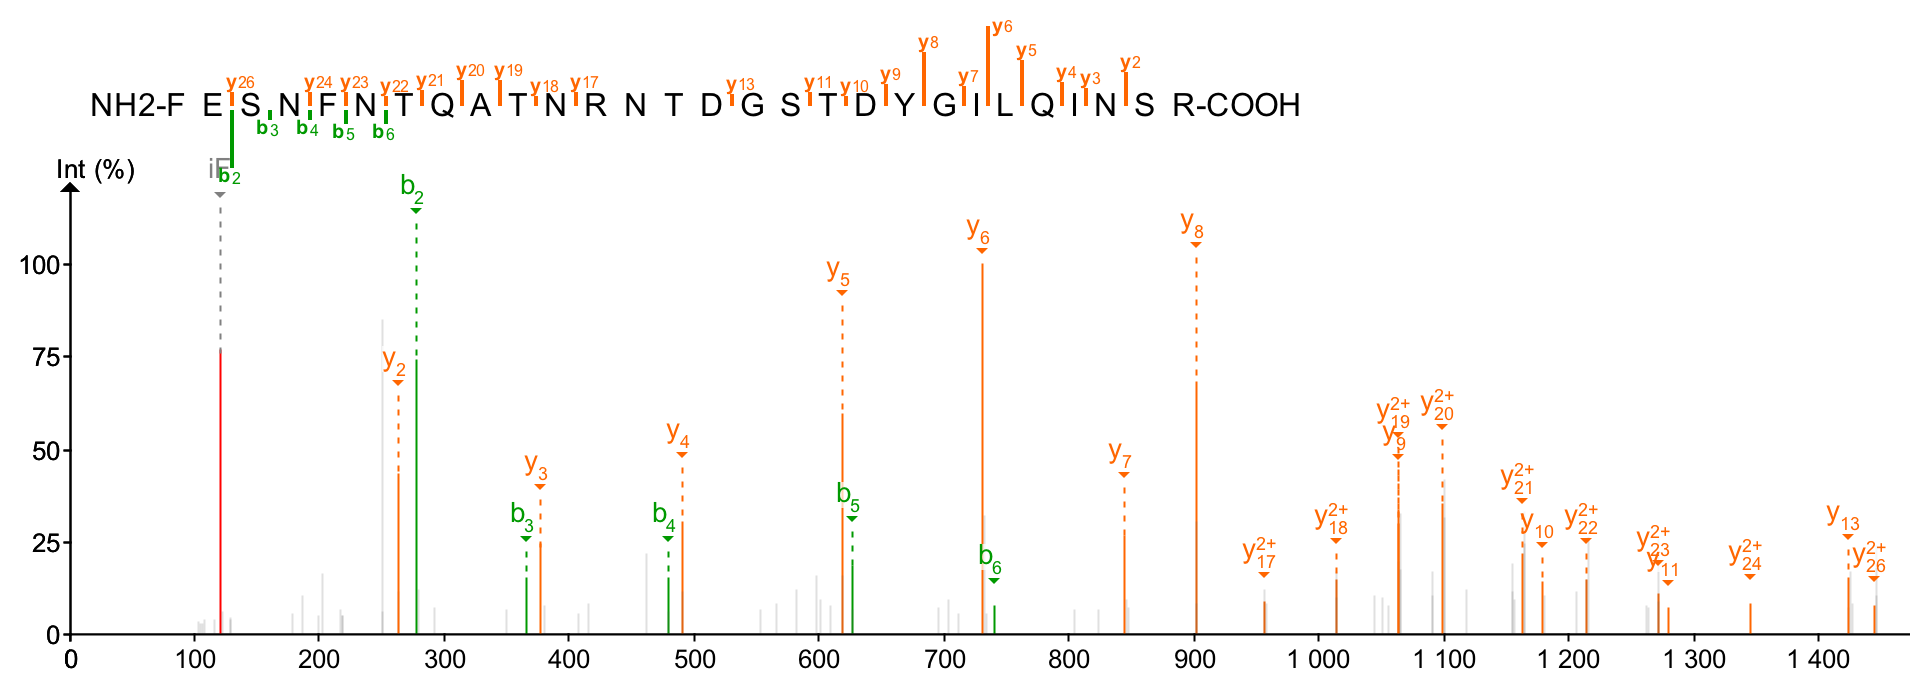
\includegraphics[width=1\linewidth]{img/fragmentation-spectrum.png}
  \caption{An annotated fragmentation spectrum of the precursor \emph{FESNFNTQATNRNTDGSTDYGILQINSR}}\label{fig:frag-spectrum}
\end{figure}

We will now discuss some specific approaches to the main phases of MS/MS analysis, putting the focus on those that are relevant for this thesis.

Nás zajímá hlavně vysoký dynamický rozsaha  vysoká přesnost.  Rozsah je při identifikaci DBs užitečný, jednak jsou to obecně informace navíc, a taky v nízkých hmotnostech bývají krátké interní fragmenty, které by mohly něco o můstcích prozradit. Má také vysokou přesnot, až pod chybovost 1ppm, což se hodí, protože přiřazování DBs je intrinsically problém s kombinatorickým výbuchem a velkou pravděpodobstí přiřazení false positive tím více, čím větší bude tolerance chyby. pomáhá to tedy snížit počet false positives.

\subsection{Sample ionization}

Save a few specific exceptions, only charged compounds are detectable by the analyser and detector in mass spectrometer; that means we have to ionize our sample in order be able to analyse it.

There are many sample ionization methods; one of the oldest is electron ionization~\cite{field2013electron}, in which the sample is first transferred to a gas phase and then bombarded with electrons. However, this method is unsuitable for large thermally unstable organic molecules, such as peptides; for proteomics work, the two most popular options are MALDI and ESI.\@

Matrix-assisted laser desorption/ionization (MALDI) is a ionization technique oft used in proteomics~\cite{caprioli1997molecular, ross1997discrimination}. In MALDI, the sample is placed on a solid light-absorbing crystalline matrix and undergoes several short focused bursts of laser light with specific wavelenghts. The light is absorbed by the sample layer which causes sample evaporation and ionization~\cite{karas1985influence}. Unfortunately for our use case, the whole ionization process has to be done in a vacuum, making it impossible to directly connect the liquid chromatography column to the spectrometer.

\subsubsection{Electrospray ionization}

For proteomics experiments that make use of liquid chromatography, electrospray ionization (ESI) is the ionization method of choice. As ESI works under atmospheric pressure, the LC colon can be connected directly to the mass spectrometer, resulting in what is usually called an  ``online'' or ``hyphenated'' LC-MS system~\cite{opiteck1997comprehensive}.

During ESI, a very fine capillary with a solution containing the sample peptides and charged ions is placed into a strong electrostatic field. Due to the influence of the field, the solution forcibly squirts out of the capillary, creating a mist of miniscule charged droplets. The solution slowly evaporates from the droplets, until eventually the repulsive electric forces inside the droplet overcome its surface tension and the droplet splits into yet smaller droplets~\cite{rayleigh1882xx}. This evaporating and splitting process repeats itself, until we are left with isolated sample ions in the gas phase~\cite{dole1968molecular,dole1968gas,fenn1989electrospray, fenn1990electrospray}.

% TODO Přidat další property, ke zopakuji, že to je napojitelné a jak je to hrozně užitečné.

For our work, two properties of ESI are important. First, ESI is a notably soft ionization technique, owing among other things to the fact it works in atmospheric pressure, which means that the sample undergoes very little to no fragmentation during the ionization~\cite{griffiths2001electrospray}. That means that the tryptides traveling to the analyser will be mostly left intact, simplyfying the subsequent analysis. The second property has to do with the typical charge of ions produced by ESI\@. Ions generated by ESI are often multiply charged~\cite{felitsyn2002origin}, bringing their \(m/z\) value down and enabling us to analyse peptides with a higher mass in an ordinary mass spectrometer setting.

\subsection{Mass analysers}

A mass analyser, together with a detector, measures the \(m/z\) ratio of a sample compound. The many existing mass analysers differ in their performance standards, the principle of function, and the sample characterstics they require to function properly.

One of the oldest mass analysers still in use is the time-of-flight (TOF) analyser~\cite{stephens1946pulsed}. It is also one of the simplest to manufacture. In TOF analysers, sample ions are accelerated with an electric field to make them travel along a path with known length. The ions with lower \(m/z\) values will arrive sooner than the ones with higher \(m/z\) values, as long as all of them are dispersed at a similar-enough point in time. Due to this requirement, TOF analysers are best suited for pulsed ionization techniques such as MALDI\@. In addition to having a relatively simple construction, TOF analysers have an excellent sensitivity and, at least in theory, their \(m/z\) range is unlimited~\cite{fuerstenau1995molecular}.

The linear quadrupole doubles as an analyser and also as a collision cell. As the name suggest, a linear quadrupole consist of four linear rods which are placed parallel to each other and arranged in a square shape, see \Cref*{fig:quadrupole}. A pair of rods sitting in diagonally opposite corners has the same polarity. However, the pairs periodically switch the polarity. An ion travelling along the rods is periodically repelled and attracted to each of the rods, its precise trajectory depending on its \(m/z\) value~\cite{paul1990electromagnetic}. In this way, ions with specific \(m/z\) values can pass through the quadrupole into a detector~\cite{paul1953neues}, while others follow an unstable trajectory and crash into one of the poles or the wall of the quadrupole.

Quadrupoles can also trap specific ions inside for prolonged period of time instead of making them simply pass through. So called linear ion traps are sometimes used as a ``staging area'' for other analysers, trapping ions and releasing them by clusters based on their \(m/z\) values further into the pipeline~\cite{mao2003h}. Another possibility is to use quadrupoles as collision cells for precursor fragmentation. For a long time, the state of the art in tandem mass spectrometry was the tripple quadrupole spectrometer~\cite{yost1978selected}; it has only lately become dethroned on the basis of accuracy by methods based on Fourier transform.

\begin{figure}
  \centering
  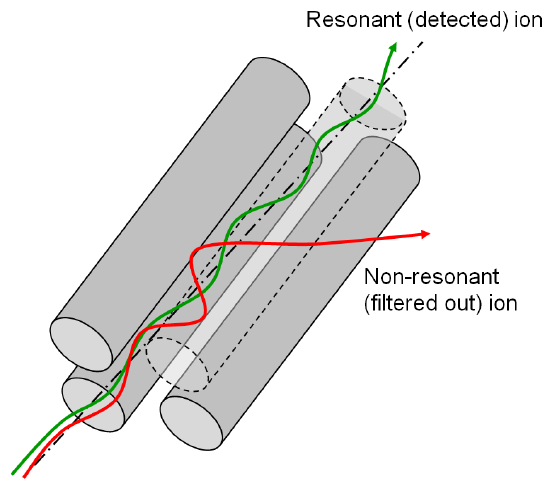
\includegraphics[width=.4\linewidth]{img/quadrupole.png}
  \caption{A quadrupole with two highlighted classes of ion trajectories. Thanks to its \(m/z\) value, the ion with green trajectory passes through the quadrupole and is ultimately detected, while the one with the red trajectory is filtered out. Image taken from~\citet{2021Mass}.}\label{fig:quadrupole}
\end{figure}

\subsubsection{Mass spectrometry based on Fourier transform}

The basis of the older of the two Fourier transform based methods, Fourier transform ion cyclotron resonance (FT-ICR), has been cocieved in 1930s by research on ion cyclotron resonance. As \citet{lawrence1932production} have shown, an ion particle in a magnetic and an electric field can be accelerated by periodically alternating the polarity of the surrounding electric field, and this in turn increases the radius upon which the particle circulates around the center of the chamber. Once the radius reaches a limit size, the particle can be detected crashing to the wall of the chamber. Later, the \(m/z\) values of the ions became measurable even without them crashing into the detector, thanks to Fourier transform that made it possible to decode the signals of passing circulating ions and calculate the \(m/z\) values from the frequencies and amplitudes~\cite{comisarow1974fourier}. This also made the measurement faster, as many ions with wildly different \(m/z\) values could be measured in parallel. Further improvements increased the mass accuracy and resolution beyond what is attainable by quadrupole analysers~\cite{amster1996fourier, easterling1999routine}.

For our work, the most important analyser type is the Orbitrap~\cite{hu2005orbitrap}. It achieves similar accuracy, resolving power and dynamic range to FT-ICR, but does not require an expensive-to-run supraconducting magnet to do so. In orbitrap the ions simultaneously cycle around the centre and oscillate along the z-axis, as is illustrated on \Cref*{fig:orbitrap}. This oscillation induces a periodically changing electrical current in the detector that is converted to a \(m/z\) spectrum of the analyte with the help of FT\@.

\begin{figure}
  \centering
  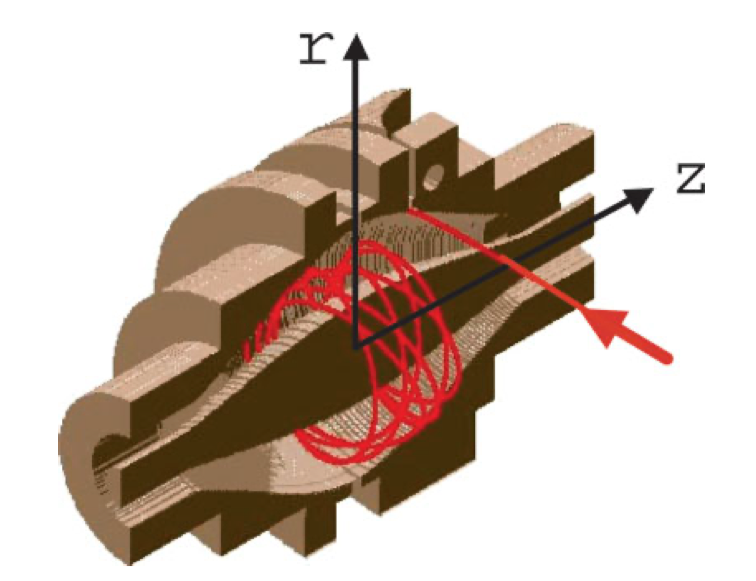
\includegraphics[width=.5\linewidth]{img/orbitrap.png}
  \caption{An orbitrap mass analyser with a typical ion trajetrory highlighted. The ion circulates around the center while simultanously oscillating along the z-axis. Image taken from~\citet{hu2005orbitrap}.}\label{fig:orbitrap}
\end{figure}

Orbitrap má vysoký dynamický rozsah a chybovost i pod 1ppm, lze jej napojit na ESI (a potažmo na LC-MSMS) je tedy pro naše účely ideální.


\subsection{Precursor fragmentation}

In tandem mass spectrometry, once the mass spectrum of the initial sample is analysed (MS1), the \emph{precursors} are selected according to their mass and fragmented, and the fragments are undergo yet another mass analysis (MS2). Again, there are many fragmentation techniques, each useful for a different type of analysis.

When aiming to observe post-translational modifications and to preserve the volatile bond connecting the PTM to the peptide, electron-capture dissociation (ECD)~\cite{zubarev2000electron} or electron-transfer dissociation (ETM)~\cite{syka2004peptide} are preferred. In ECD a multiply positively charged precursor ion is hit by a beam of low-energy electrons, while in ETD the electron transfer is induced by negatively charged reagent ions, both of these ultimately leading to the creation of a radical cation and amine backbone bond cleavage, resulting in the creation of \(c\) and \(z\) ions, as illustrated on \Cref*{fig:fragment-types}. These methods require a multiply-charged precursor ion, because the absoption of the elector lowers the overall charge by 1, making singly charged precursor ions undetectable.

\begin{figure}
  \centering
  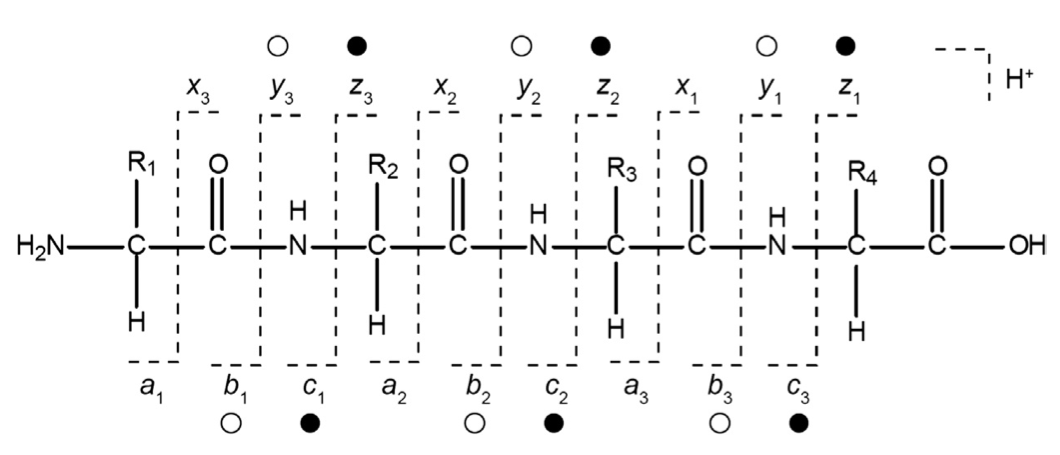
\includegraphics[width=.75\linewidth]{img/fragment-types.png}
  \caption{A singly positively charged peptide with annotated fragmentation types. Signature CID b/y ion fragments are marked with open circles, while the typical ECD and ETD c/z ion fragments are marked with filled circles. Image taken from~\citet{hart2014review}.}\label{fig:fragment-types}
\end{figure}

The fragmentation method we focus on in this work, however, is collision-induced dissociation (CID). It has a different fragmentation signature compared to the abovementioned methods (see \Cref*{fig:fragment-types}), and it doesn't preserve PTMs nearly as well as they do. Thankfully, DBs are not as labile as the bonds connecting PTMs to the peptide, and thus CID can be safely used to produce fragments from breptides [citace]. A similar fragmentation signature to CID can also be obtained by infrared multiphoton dissociation (IRMPD)~\cite{oomens2006gas}. Because IRMPD, and the related UV-MPD, do not require collision gasses to be present for the fragmentaion, they are well suited for analysers operating under high vacuum, such as FT-ICR\@.

\subsubsection{Dissociation based on collision with neutral gas molecules}

Two common fragmentation methods fall under the umbrella of fragmenting by collision with neutral gas: collision-induced dissociation (CID) and higher-energy C-trap dissociation (HCD). Both of them make the accelerated precursor ions collide with neutral gas molecules, ultimately leading to its fragmentation, but use different instrumentation to reach this goal, and have different performance characteristics in different contexts.

The principle of function is not the only thing these two methods have in common; they also share a big portion of the fragmentation signature~\cite{michalski2012systematic}. In both CID and HCD the dissociation process usually takes place at the more labile bonds, such as the ones connecting PTMs~\cite{quan2013cid}, or peptide bonds in the precrusor backbone, resulting in the generation of \(b\) and \(y\) fragment ions (see \Cref{fig:fragment-types}).\footnote{The fact that many PTM bonds are preferentially dissociated during CID is usually seen as undersirable. However, in our case it simplifies the analysis, as we can safely ignore PTMs and reduce the combinatorial complexity.} As a side-effect of the dissociation, a small neutral molecule sometimes breaks off of the fragment, lowering its total mass value without affecting its charge. This dissociated molecule is termed the \emph{neutral loss}; during CID and HCD, the most common neutral losses are water and amonia from the fragment N-- and C-- termini, and various other small molecules from specific amino acid side-chains.

The similarities do not end there: HCD and a specific subset of CID, a so called beam-type CID, also share a method of inducing the collisions. Precursor ions travel in a beam through a collision cell, and collide with the gas molecules along the way~\cite{xia2006ion}. Because of this passage through the cell, the precursor ions are sometimes dissociated more the once, resulting in the generation and detection of \emph{internal ions}. Many of the internal ions begin with a proline~\cite{michalski2012systematic}, revealing that the double cleavage event prefers some amino acids to others.

The beam-type CID is often connected to a quadrupole analyser (being a quadrupole itself in a 3-quadrupole mass spectrometer), however, which can sometimes make it hard to interpret these spectra due to its relatively low accuracy. As shown by \citet{michalski2012systematic}, ion trap CID, unlike the beam-type variant, doesn't lead to the creation of internal ions. Furthermore, it has limits regarding the containment of molecules below a certain mass threshold, leading to a mass cutoff~\cite{louris1987instrumentation}.

In the year 2007, the HCD dissiociation technique has been introduced~\cite{olsen2007higher}, combining the richer sequence information~\cite{xia2006ion} and lower mass cutoff of beam-type CID with the superior resultion capacity and accuracy of the orbitrap analyser; the accuracy was reported to be in the sub 1 ppm levels by the original paper. Data we use in this thesis are generated with HCD\@, because the high accuracy of its MS2 spectra makes it easier to filter out false positives that occur naturally during in silico matching of the spectra due to the combinatoric nature of the problem. Furthermore the detected internal ions can occasionaly be useful when determining the connectivity of complex DB configrations. Because the HCD fargmentation pathways are key to our work, we will discuss them in more detail below.

\paragraph{Fragment types} The fragment types of a very pure sample protein were nicely summarized by \citet{michalski2012systematic}. Ions of \(b\) and \(y\) type comprise most of the spectral intensity (54\%, see \Cref{fig:hcd}), together with \(b\) ions with \(\ce{CO}\) neutral loss that are interchangeable with \(a\) ions. The ions themselves have different distributions, \(y\) ions being the most abundant. Other neutral loss ions, be it a loss of water, amonia, or an amino-acid-specific small molecule\footnote{If specific amino acid neutral losses are of interest, the wonderful review by~\cite{paizs2005fragmentation} lists many of them.}, together with internal ions, can be attributed a quarter of the total fragment intensity. Immonium ions account for 6\% of the intensity, totaling 85\% intensity that can be explained with the current understanding of HCD fragmentation pathways. For a visual overview of the many different HCD fragmentation types, please refer to \Cref{fig:fragment-types-hcd}.

\begin{figure}
  \centering
  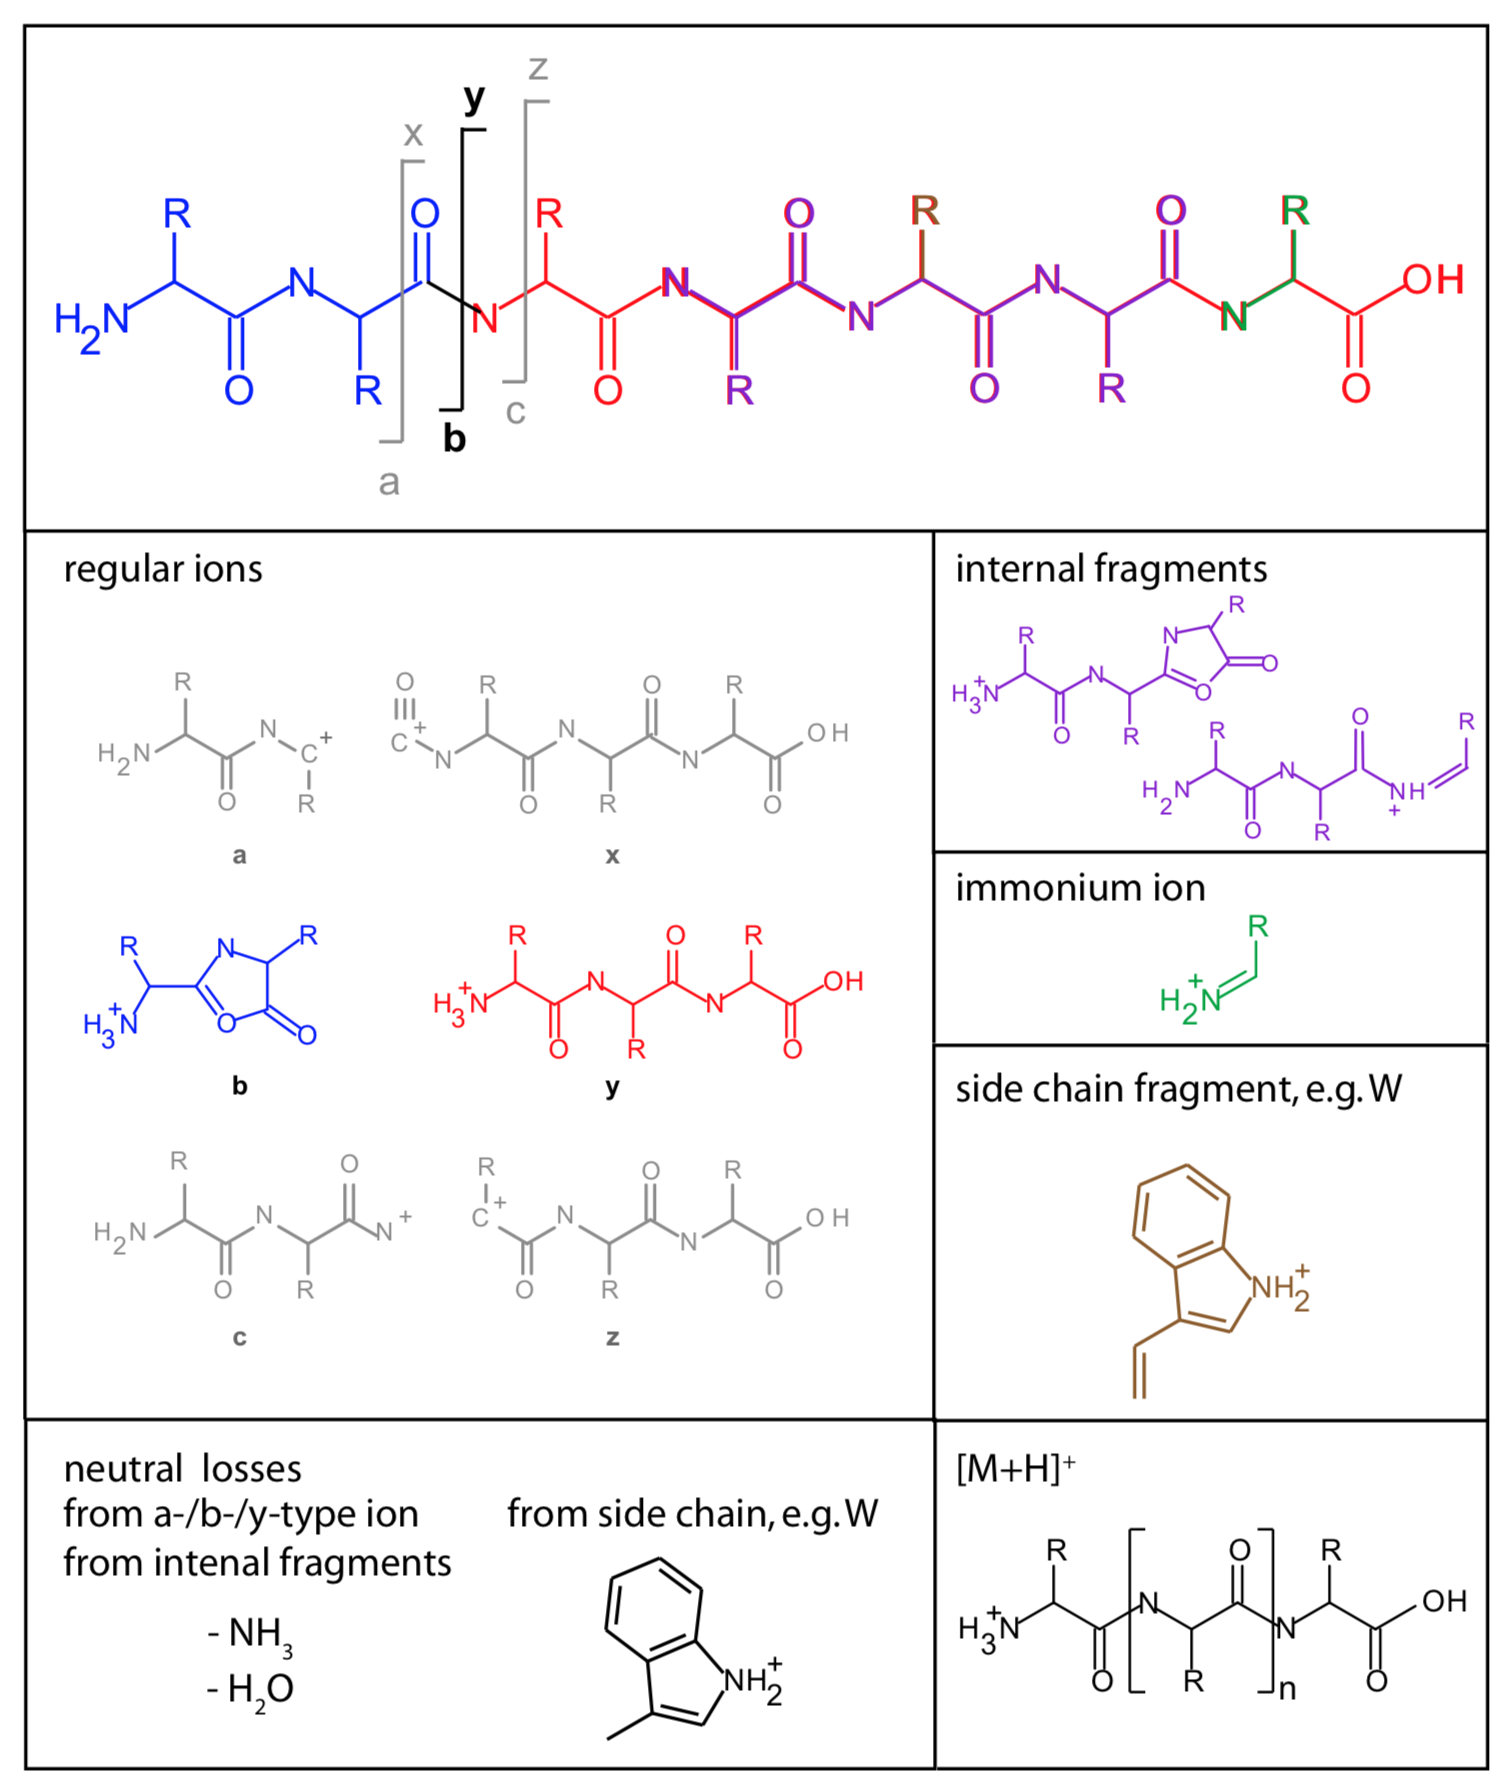
\includegraphics[width=.9\linewidth]{img/fragment-types-hcd.png}
  \caption{During HCD, \(b, y\), and to a lesser extent \(a\), ions are the most common, together with internal ions and immonium ions, and their counterparts with neutral losses. Image taken from~\citet{michalski2012systematic}.}\label{fig:fragment-types-hcd}
\end{figure}

\begin{figure}
  \centering
  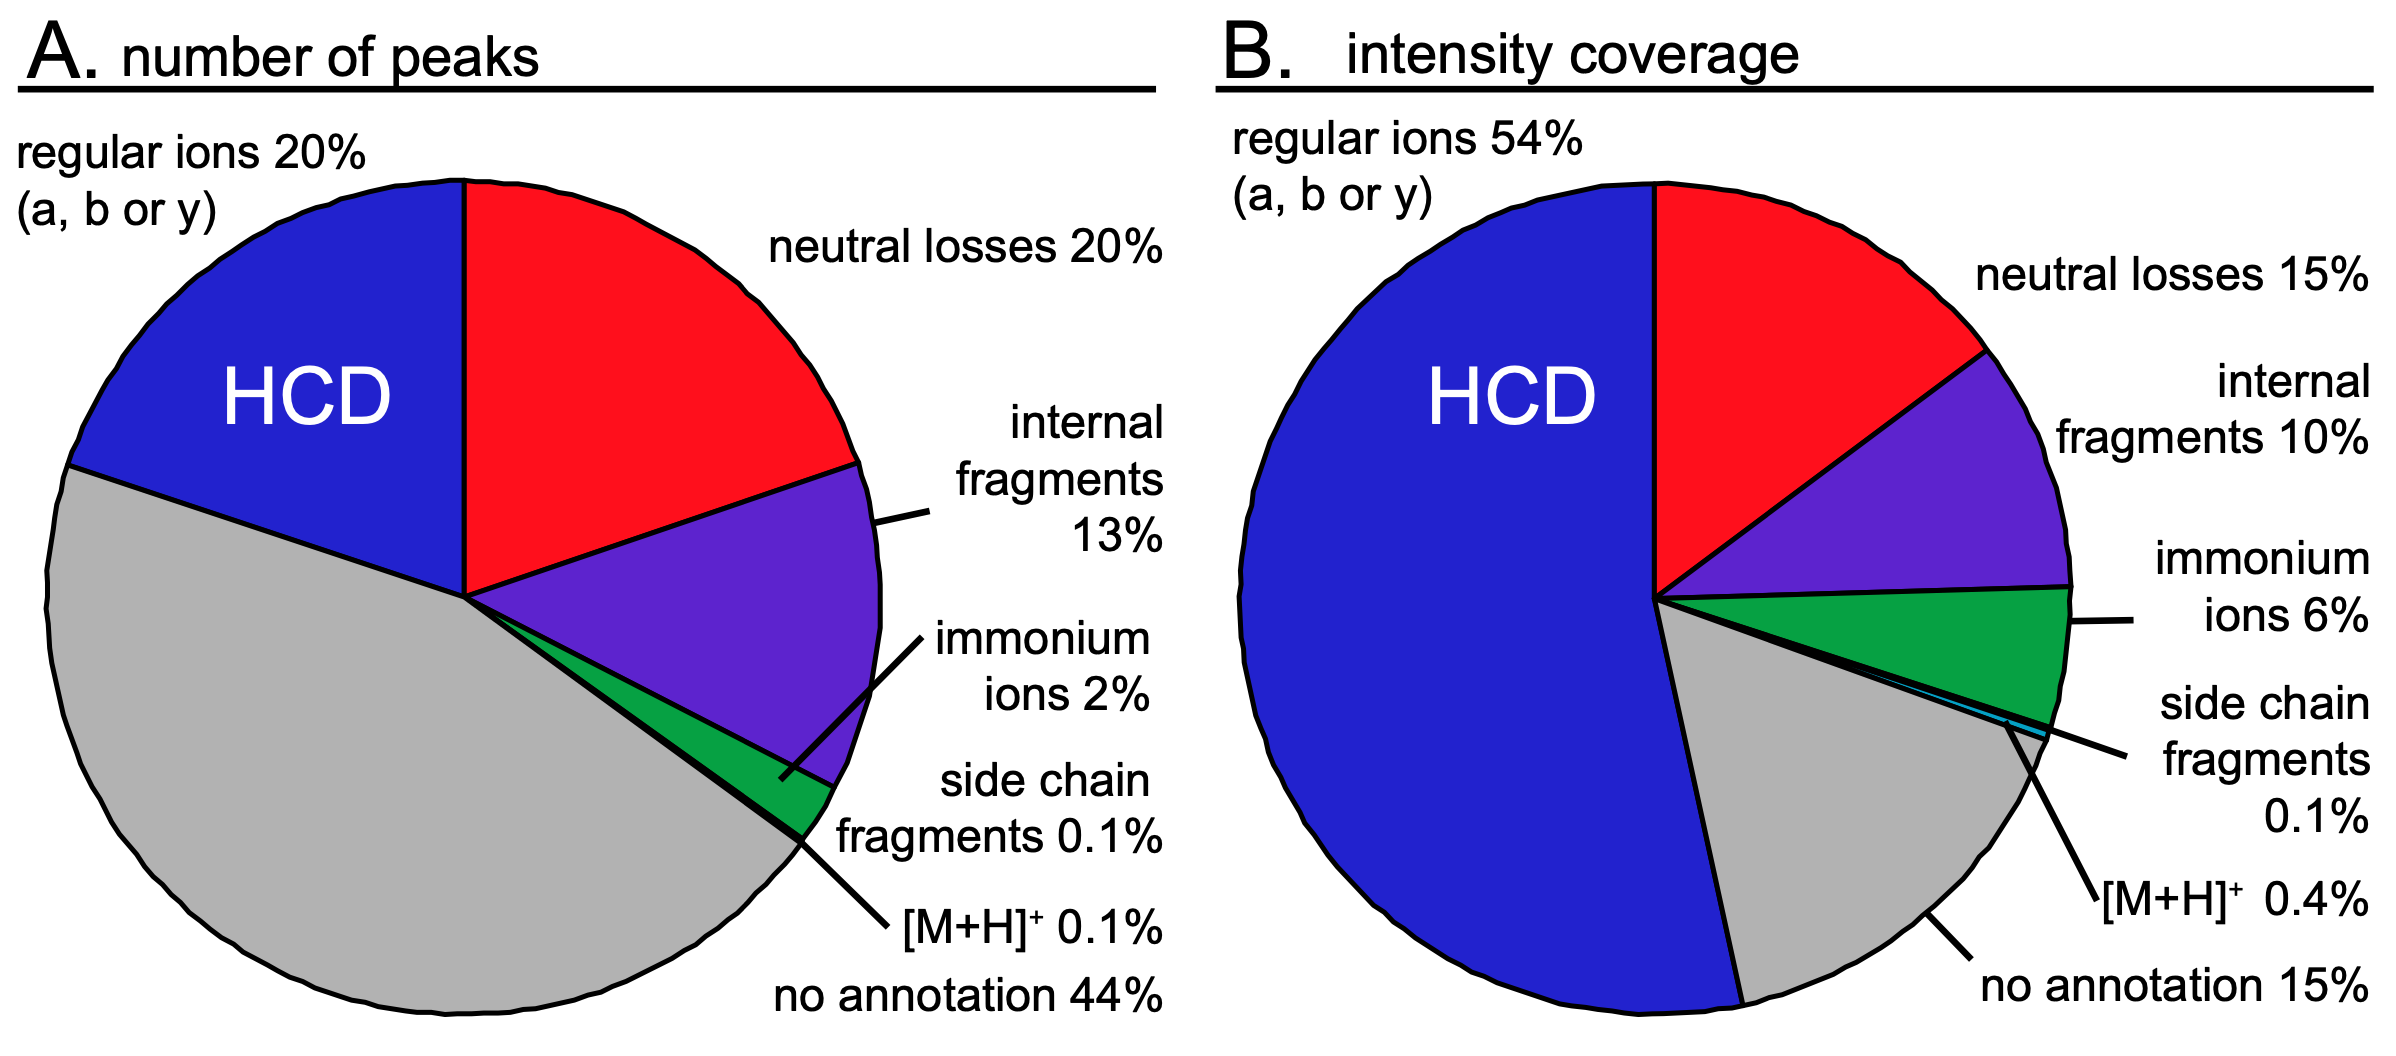
\includegraphics[width=.9\linewidth]{img/hcd.png}
  \caption{(B) The regular \(b, y\), and \(a\) ions take up 54\% of the measured spectral intensity. Another 25\% is explained by fragments with neutral-loss and internal fragments, and another 6\% by immonium ions. Together, those four account for 85\% of the measured intensity. It is true that almost a half of the peaks are still left unexplained (A), however, given all of these fragments have to split the remaining 15\% of intensity, they are probably rather rare and are only of moderate importance. Image taken from~\citet{michalski2012systematic}.}\label{fig:hcd}
\end{figure}

\paragraph{Charge} Coming from ESI-ionized precursors, fragments can be and indeed often are multiply charged~\cite{katta1991use, michalski2012systematic}; the only real limit of the fragment charge is the charge of its precursor. Of course, uncharged fragments are undetectable by the mass spectrometer. According the research on CID of crosslinked peptides by \citet{giese2016study}, most of the crosslined fragments were found to have a positive charge of at least 2, while an overwhelming majority of linear fragments had a positive charge of 1. Their results are illustrated on \Cref{fig:crosslink-charge}.

\begin{figure}
  \centering
  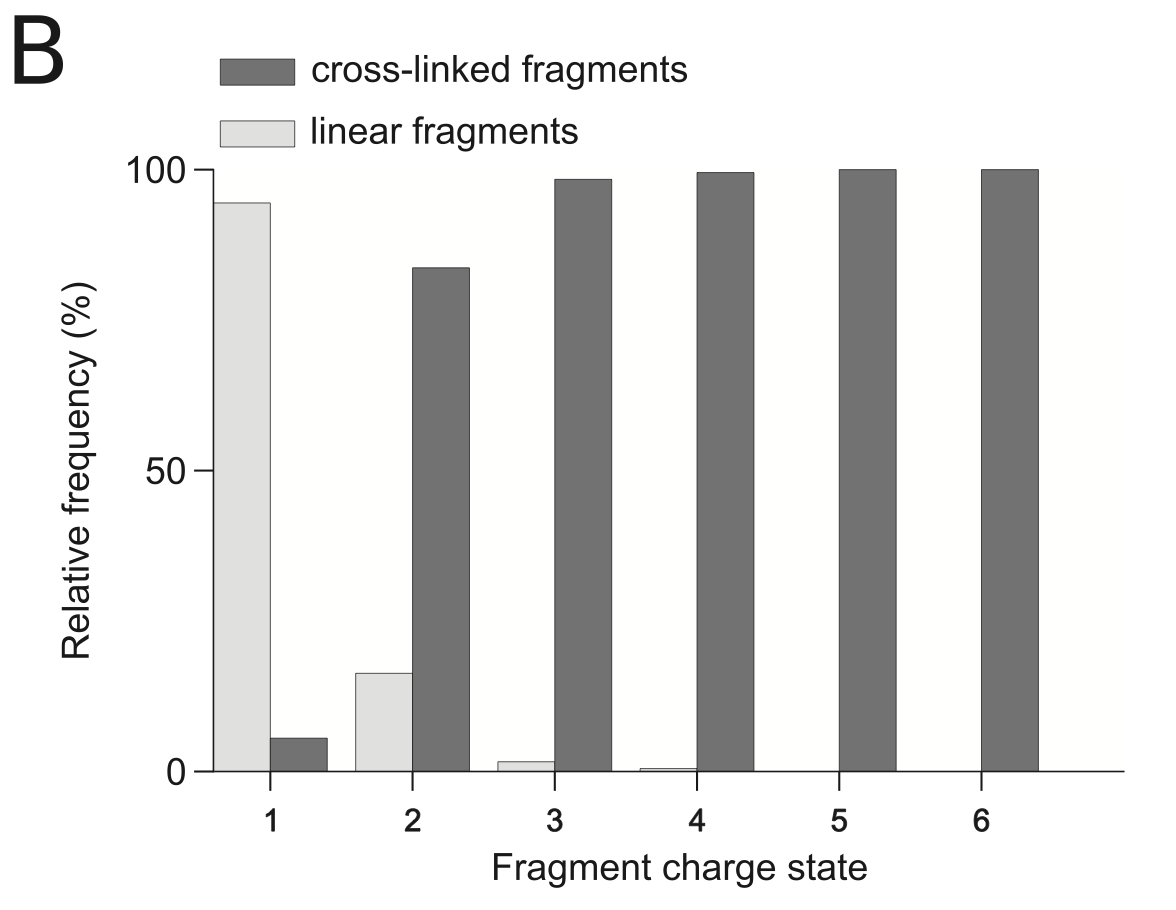
\includegraphics[width=.5\linewidth]{img/crosslink-charge.png}
  \caption{Most linear fragments have charge 1, and most crosslinked fragments have a charge of 2 or higher. Image taken from~\citet{giese2016study}.}\label{fig:crosslink-charge}
\end{figure}

The fragmentation pathways are complicated enough even without the presence of DBs, and the addition of peptide crosslinks complicates the matter further. We have to take into account the alkylation of non-bonded cysteines during the analaysis; the DB can be cleaved during the dissociation, resulting in fragments roughly resembling the fragmentation pathway of each connected peptide in the original precursor. If left intact, the crosslinks between precursors (or within one precursor) widen the possibilities of attainable mass values considerably.

\paragraph{Disulphide bridges} Although DBs are not affected by low-energy CID as much as the other PTMs~\cite{paizs2005fragmentation, lioe2007novel}, in high energy collision fragmentation, cleavage of the S-S bond can be observed with a higher probability~\cite{bean1992characterization}. The cleavage of the bond can result in the formation of an asymetrical distribution of mass on the two cysteines~\cite{zhang2006mapping}, that has been nicely ilustrated by \citet{tsai2013mass}, see \Cref{fig:disulfide-bond-cleavage-assymetry} for details. The sole presence of a DB influences the fragmentation pathway of the whole peptide; \citet{mormann2008fragmentation} reports a low but detectable signal of peptide backbone cleavages in the bonds instide S-S loop of an internal DB, while \citet{clark2011collision} reports a higher frequence of internal ions. The latter complicates the analysis noticeably as we have to take all combinations of cleavage positions from all interlinked peptides in the precuror, but also in theory allows us to differentiate between different configurations of intra-peptide bonds, such as those on \Cref{fig:intrapeptide-bonds}.

\begin{figure}
  \centering
  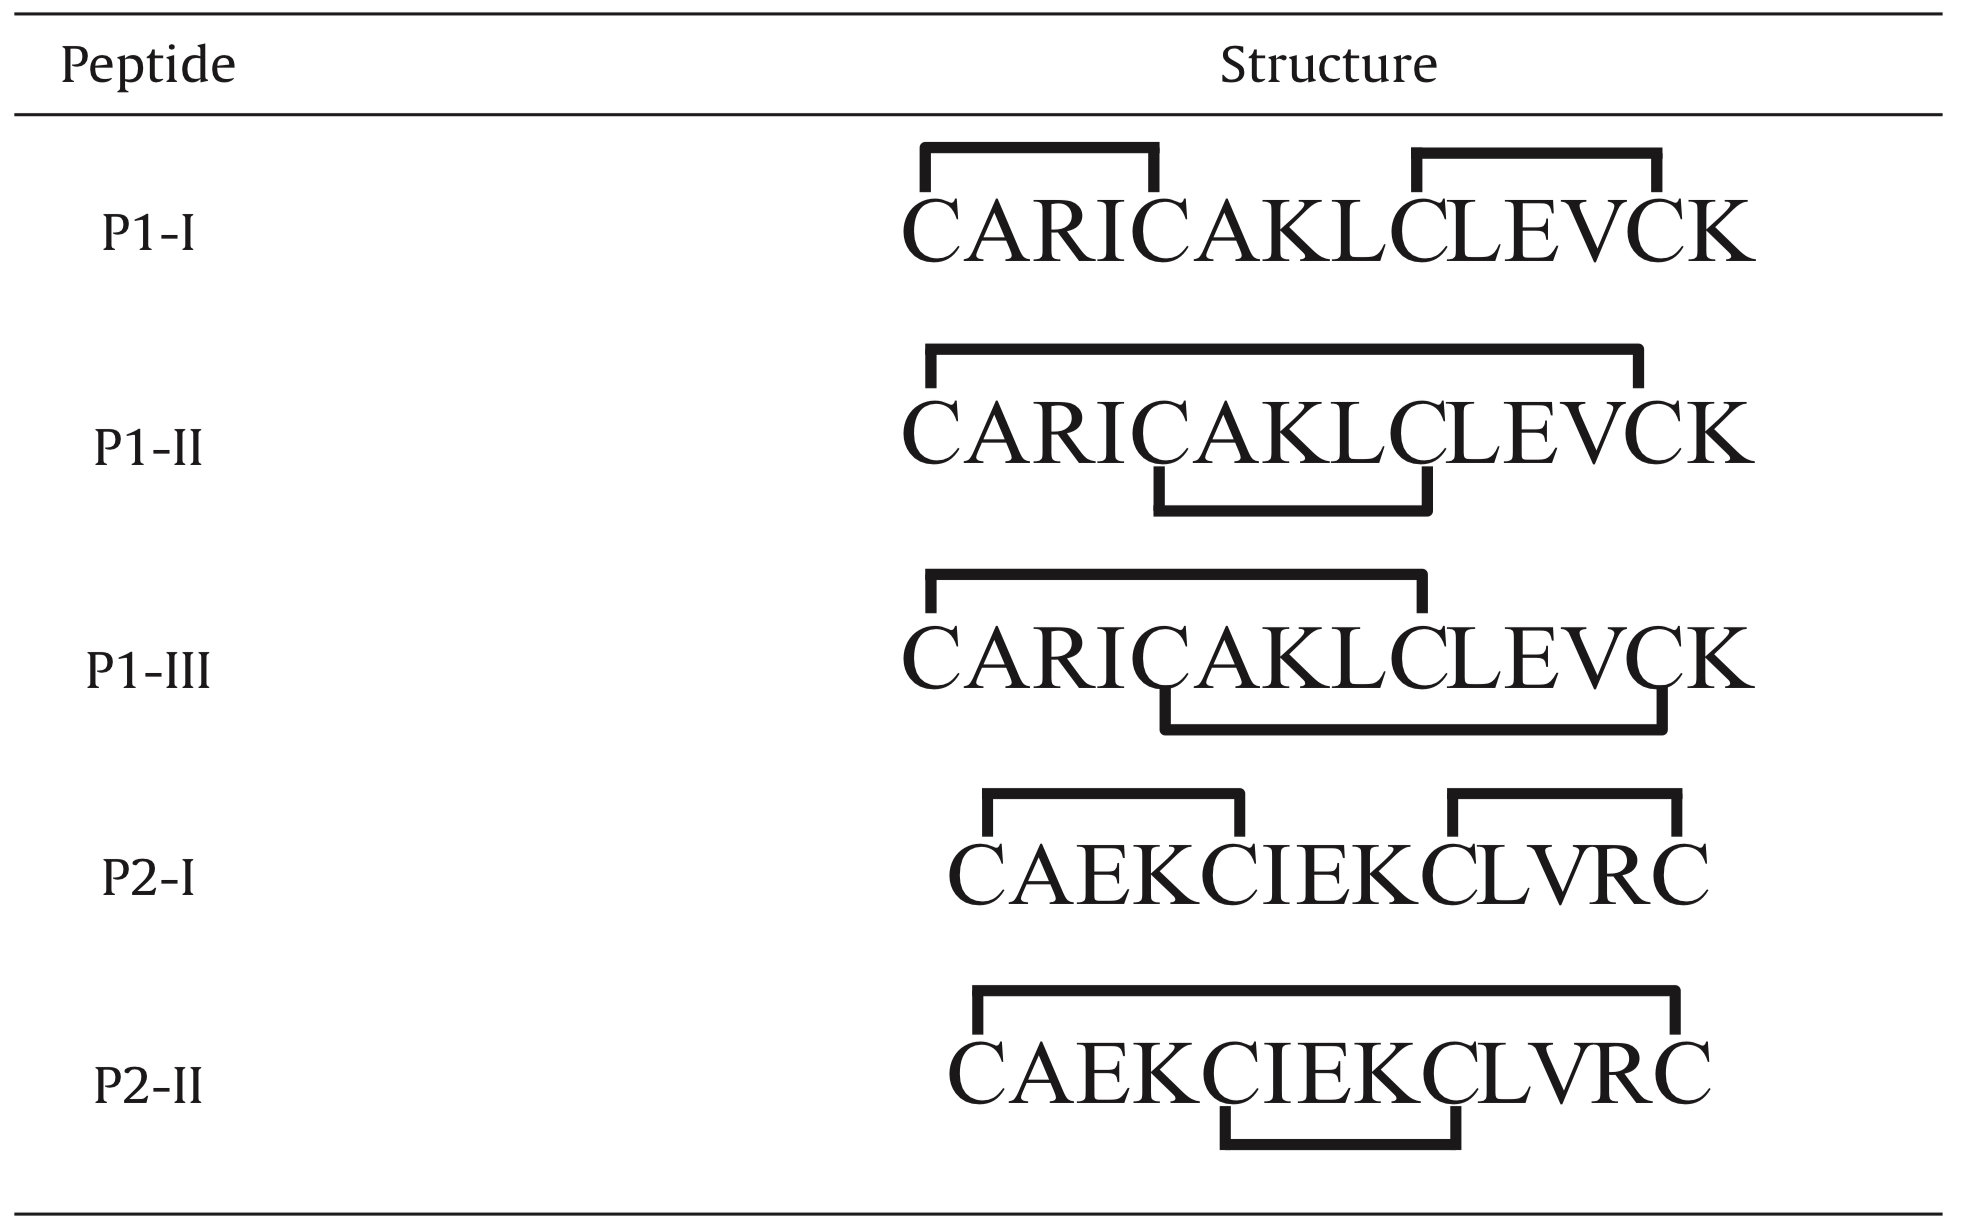
\includegraphics[width=.5\linewidth]{img/intrapeptide-bond.jpeg}
  \caption{An example of different possible configurations of intra-peptide DBs. Image taken from~\citet{durand2013tandem}.}\label{fig:intrapeptide-bonds}
\end{figure}

\begin{figure}
  \centering
  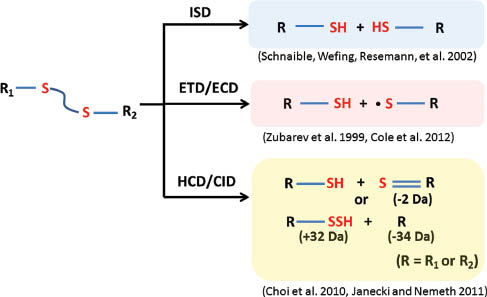
\includegraphics[width=.6\linewidth]{img/disulfide-bond-cleavage-assymetry.jpg}
  \caption{Under different dissociation strategies, DBs manifest different cleavage characteristics. Under CID, the cleavage results into two possible assymetrical mass distributions. Image taken from~\citet{tsai2013mass}.}\label{fig:disulfide-bond-cleavage-assymetry}
\end{figure}

To recapitulate, HCD fragmentation pathways of non-crosslinked peptides are relatively well-understood. However, the presence of DBs results in complex fragmentation patterns that are hard to analyze. The existing methods for DB identification thus usually involve a lot manual work, or do the bulk of the analysis in silico, but require the researcher to manually discard the many generated false positive matches afterwards. We briefly review some of these methods in the next section.

\section{Breptide spectra interpretation}

This section concerns itself with the existing methods aiming to determine the quantity and position of DBs in a protein using tandem mass spectrometry. We focus on the computational methods, and finally formulate the precise task that this thesis is trying to solve together with a simple complexity analysis.

As noted by \citet{lakbub2018recent}, there are two main types of DB characterization. Profile comparison methods make use of two samples, one reduced with the DBs removed and one nonreduced that has its DBs still intact. Differential analysis is then deployed on a chromatogram profile of these two samples to determine which peptides are in the nonreduced sample, but not in the reduced one. Those peptides are suspect of being breptides and are further analyzed by MS/MS. Intact analysis methods only data from the nonreduced sample. Thus, they simpler from the sample preparation standpoint, but have to work with less information than the profile comparison methods.

In each of the both categories, the protocols further differ in the choice of of sample separation, ionization, and fragmentation methods, the choice of mass analyzer, and whether the bulk of the analysis is performed manually or automatically~\cite{lakbub2018recent}. Some of the software for automatic DB characterisation is reviewd below; for the sake of completness, an example of a partially-manual method now follows.

\citet{wu2009mass} propose an intact analysis method based on LC-MS/MS with ETD\@. The prepared breptides are measured on MS1 and fragmented by ETD\@. During ETD the DBs are dissociated, resulting in fragmentation spectra with two prominent peaks that represent the original peptides that were connected with the DB\@. Fragments from these two peaks are put into an MS3 step with CID fragmentation to gain sequence information about them. This sidesteps the problem of not having data from the non-bound peptides in the intact methods. Software for fragment mass searching and matching is used, but because it is not made with DB research in mind, the method requires manual intervensions when interpreting internal ion peaks, or when the peptide assignment to the birdgetide spectra based on the two prominent ETD peaks is not clear cut. Specialized sofrtware dedicated for DB cahracterisation is reviewed in the next section.

\subsection{Current computational approaches}

Dedicated DB characterisation software usually only needs data from nonreduced samples, however, there are some commercial options that offer the possibility to add data from reduced samples as well, such as PepFinder and BioPharma Finder, as noted by \citet{lakbub2018recent}. Refer to the same publication for a more comprehensive list of past and current manual and compuational DB characterisation methods.

SimXL is tool for general peptide cross-linking analysis~\cite{lima2015sim}, including DBs~\cite{cui2019comprehensive}, seemingly without having a preferred fragmentation method. SimXL has three main differentiating factors. Frist is the user-friendly UI that allows the reasearchers to view not only the interpreted results, but also the annotated data based on which they were computed. Second is its search space reduction heuristc based on the presence of a reporter ion~\cite{iglesias2010identification}, a peak that is specific to the fragmentation spectra of crosslinked precursor; in the context of our task, alkylated cysteines could be possibly interpreted as reporters~\cite{wei2020identification}. Finally, SimXL employs a further search space-reduction heuristic based on dead-end modifications, but we believe it is probably inapplicable in the context of DB characterisation.

A popular method by \citet{liu2014facilitating} comes with a whole recommended research protocol. Samples are digested with pepsin to avoid the DB scrambling that is typical low-pH for tryptic digestion, fragmented with ETH followed by HCD, together called \emph{electron transfer higher energy dissociation} (EThcD), and finally analyzed with SlinkS, a dedicated DB matching algorithm. As mentioned previously, it is possible to extract information about the peptides contituting the precursor ion from the ETH fragmentation spectra. The HCD step is employed in order to gain sequenec information about these peptides, similary to how MS3 has been used in~\cite{wu2009mass}.

Ultimately, thanks to EThcD, two peaks corresponing to the precursor peptide pair are identified in each fragmentation spectrum, and the whole precursor match is scored by scoring the other individual fragments now that we know from which precursor they (allegedly) came. The method is elegant, but its main shortcoming is the fact that it only works with dipeptide precursors; it also ignores fragments with neutral loss and internal ion fragments. That makes it impossible to identify some of the more complicated DB configurations.

In fact, all of the aforemetioned methods should be able to match simple interpeptide DBs, but they reportedly struggle with more complex intrapeptide bonds or intertwined interpeptides~\cite{lakbub2018recent}; some of those can be seen on \Cref{fig:bond-types}. A wide array of approaches to DBs is offered, leading to a yet wider array of recommended sample preparation and fragmentaion protocols. We conclude that computational DB characetrisation is a hard problem to solve, a notoin we further formalize in the next section.

\begin{figure}
  \centering
  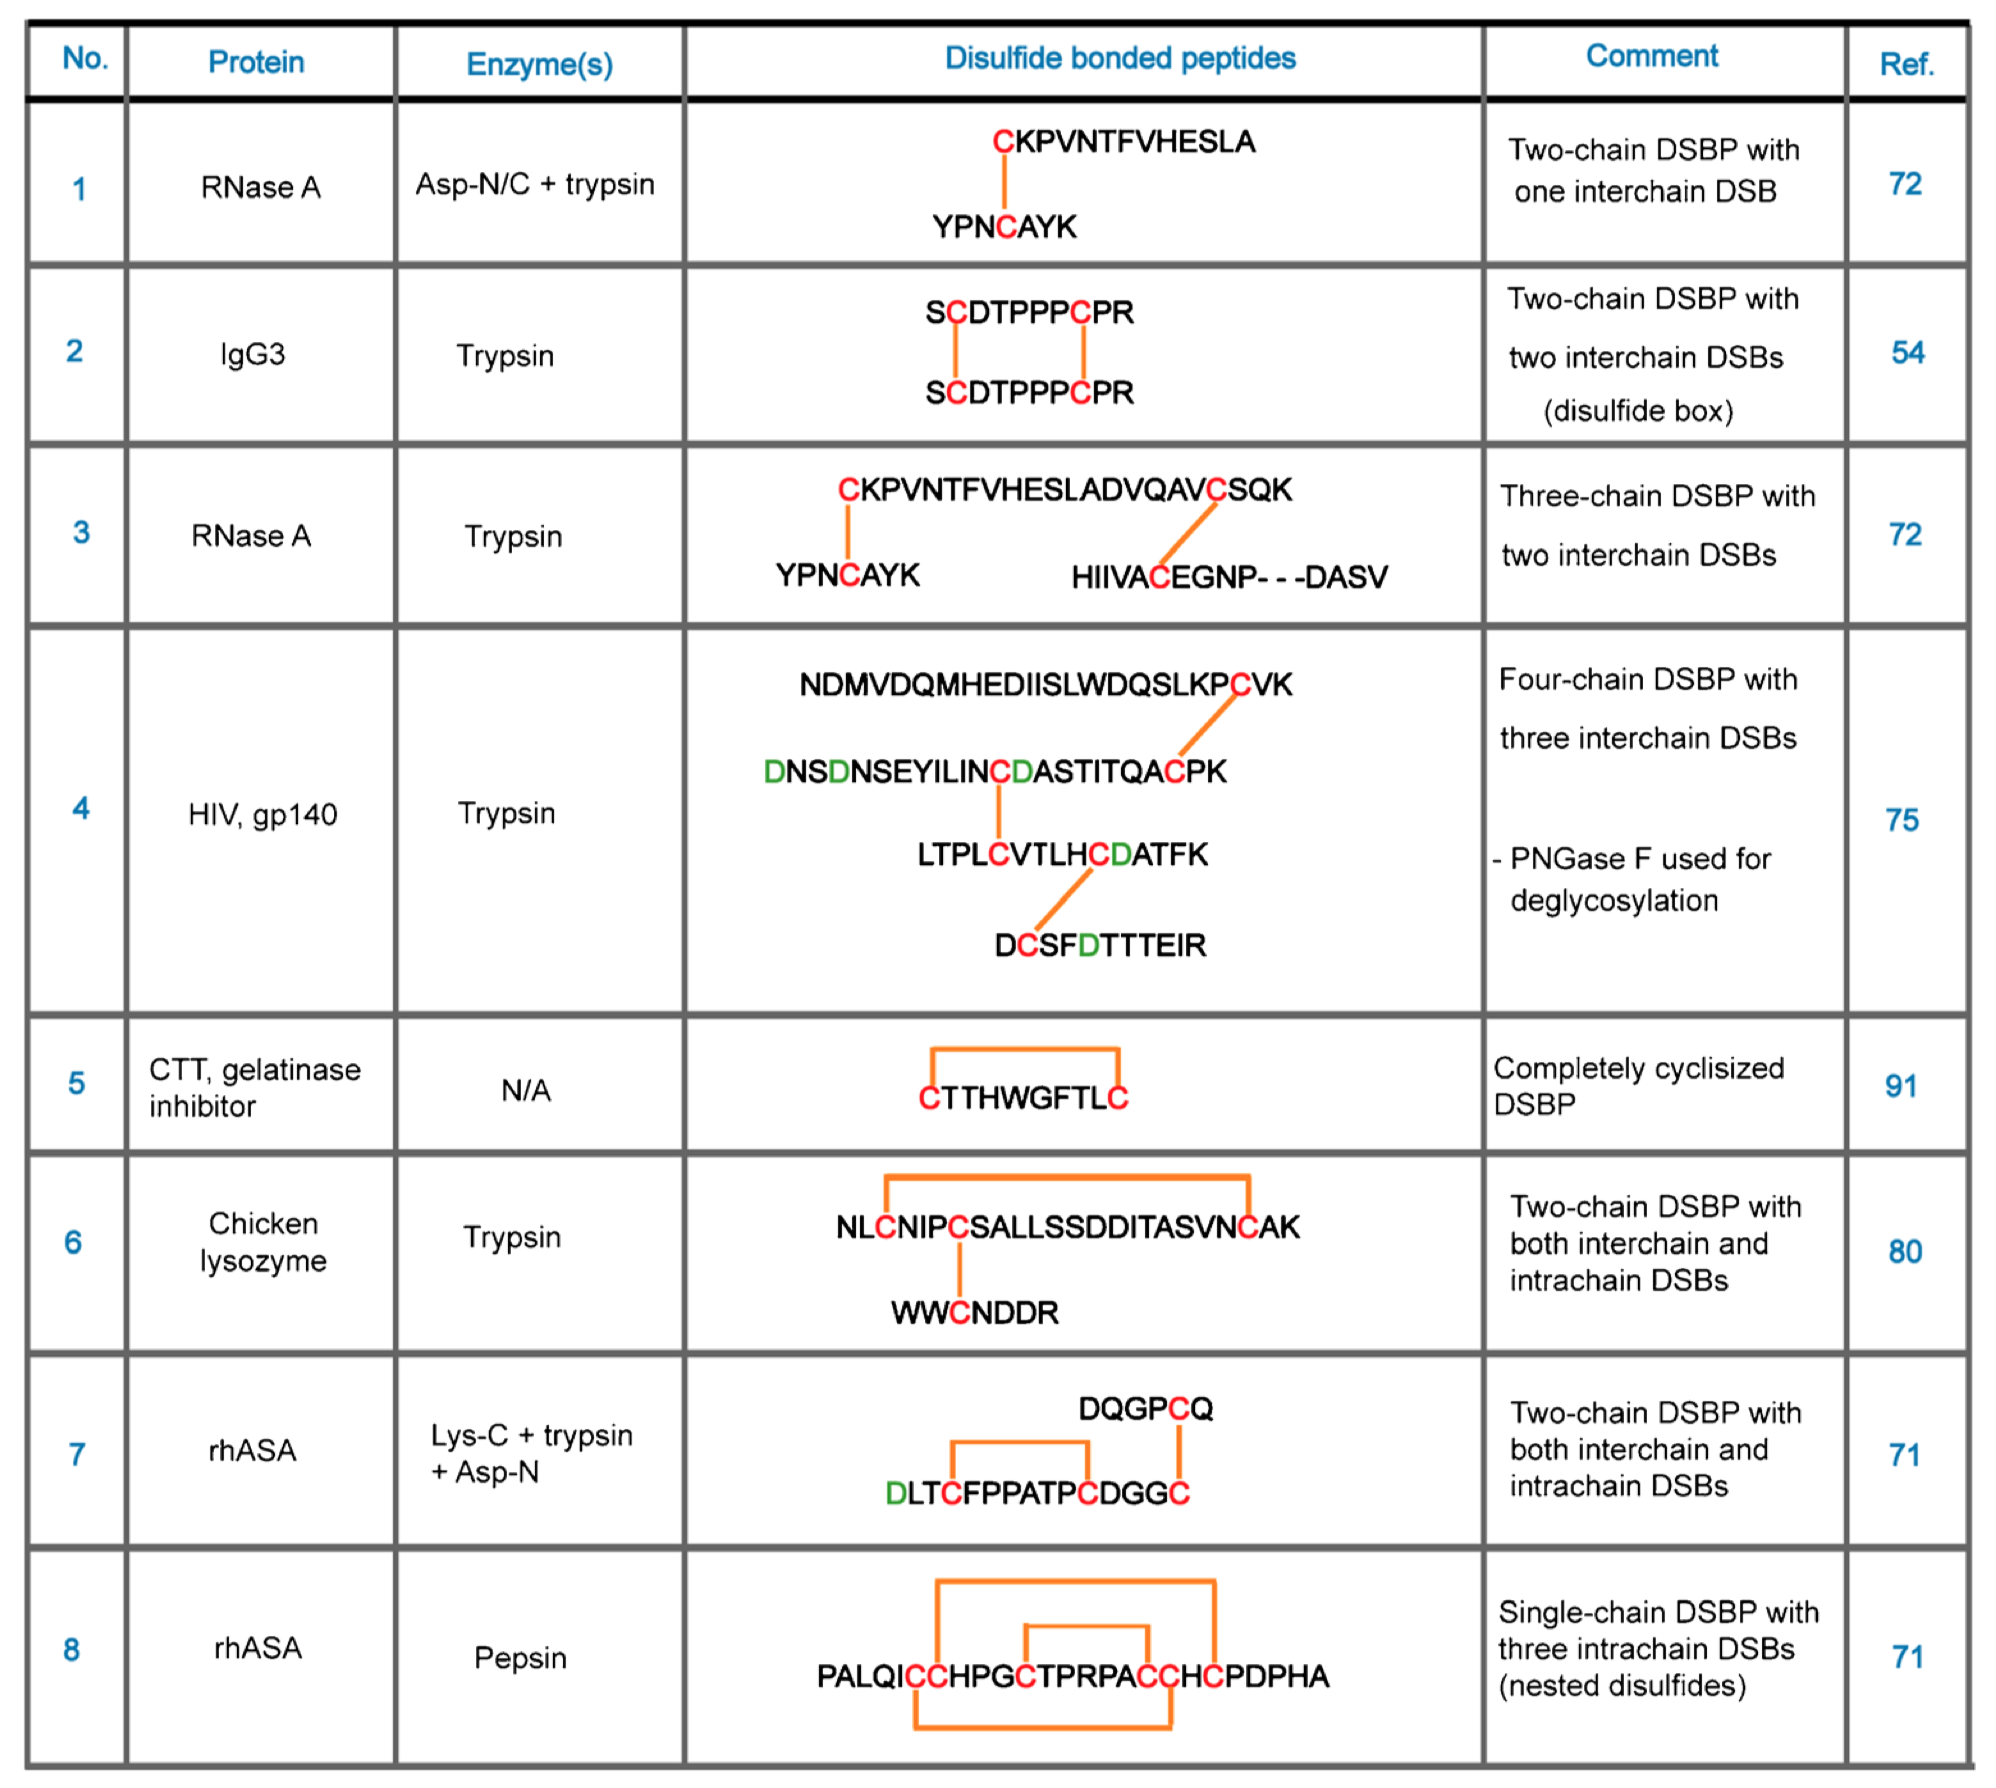
\includegraphics[width=1\linewidth]{img/bond-types.png}
  \caption{Illustrative examles of different ways peptides can be connected by disulfide bonds, ranging from realtively simple examples (1, 3, 5) to complex multipeptide or multibond configurations (4, 8). The more complicated configurations proved to be hard to characterise computationally. Image by~\citet{lakbub2018recent}. (DSB = disulfide bond, gp140 = glycoprotein 140, rhASA = recombinant human arylsulfatase A)}\label{fig:bond-types}
\end{figure}


\subsection{Problem statement and complexity}

Undisputably, the problem of determining the characteristics of DB linkages in proteins is hard. From biochemical point of view, already sample preparation poses a challenge; there is a need to minimize DB scrambling, but at the same time have the protease be as specific as possible to simplify the subseqeucnt analysis.

Another unresolved problem is the choice of dissociation method. ETD spectra offer the information about the constituent peptides, which is undisputably useful when assigning precursor peptides. On the other hand, CID-based approaches have access to richer but more complicated fragmentation spectra, including interlinked fragments and internal ions with intact DBs; these are useful for precise pinpointing of the DB location.

To continue this discussion further, we need to be specific about the precise task we are attempting to solve. In this thesis, the task is to identify precursor breptides in provided mass-spectrometric data, score them, and use the calculated scores to weigh the information the precursors provide about a part of the analyzed protein cysteines. The scoring will be done based on how well will the a in silico generated fragments of the assigned breptide match the measured fragmentation spectrum. Thus is the split into two similar subproblems: precursor matching, and then scoring by fragment matching. We will describe theoretical complexity of fragment matcing below, and most of the remarks will carry over to precursor matching as well. While the scoring paradigm itself is a very complicated thing, the main algorithmic complexity comes from the matching of fragments which is a prerequisite for the score calculation step.

\subsubsection{A simplified variant of the task}

We are provided a precursor \(R\) comprising of \(n\) residues with integer masses, interlined with DBs and peptide bonds, and a target integer fragment mass \(f\). Our task is to find all fragment ions from \(R\) whose mass exactly matches \(f\).

% TODO PRecursor graph je variant graph

We can model the precursor as a graph \(G_R = (V, E)\) with weighted nodes, where \(|V|  = 1\ldots n\) and \((i, j) \in E\) if and only if there is a peptide or a disulfide bond connecting  the \(i\)-th and \(j\)-th residue in \(R\). The weight \(w_i\) of the vertex \(i\) is the mass of the corresponding \(i\)-th residue in the precursor. We will call this graph the \emph{precursor graph of the precursor} \(R\). Even though the bonds in \(R\) are constrained in terms of connectivity --- there can be at most one DB connected to a given residue, and at most two peptide bonds --- \(G_R\) can still in theory be a relatively complex non-planar graph, as illustrated on \Cref{fig:nonplanar}.

To solve the task, we need to find all contiguous subgraphs of the precursor graph of \(R\) in which the sum of weights is exactly \(f\), a problem that is usually called the exact weight subraph problem~\cite{abboud2013exact}, or, in our case, an exact weight \emph{connected} subgraph problem. A well-studied closely related problem called the maximum weight connected k-subgraph problem was shown to be NP-hard on general graphs, and even on planar and bipartite graphs with integer weights~\cite{hochbaum1994node}; the same authors propose a polynomial-time \(O(k^2n)\) dynamic programming algorihm for the a restricted version of the problem searching for subgraphs in trees. The exact weight conencted subgraph problem has not been studied quite as thoroughly, but we think it is safe to assume that its complexity will not be much lower. In other words, in the context of our not-necessarily-planar precursor graphs, the problem is probably NP-hard.

\begin{figure}
  \centering
  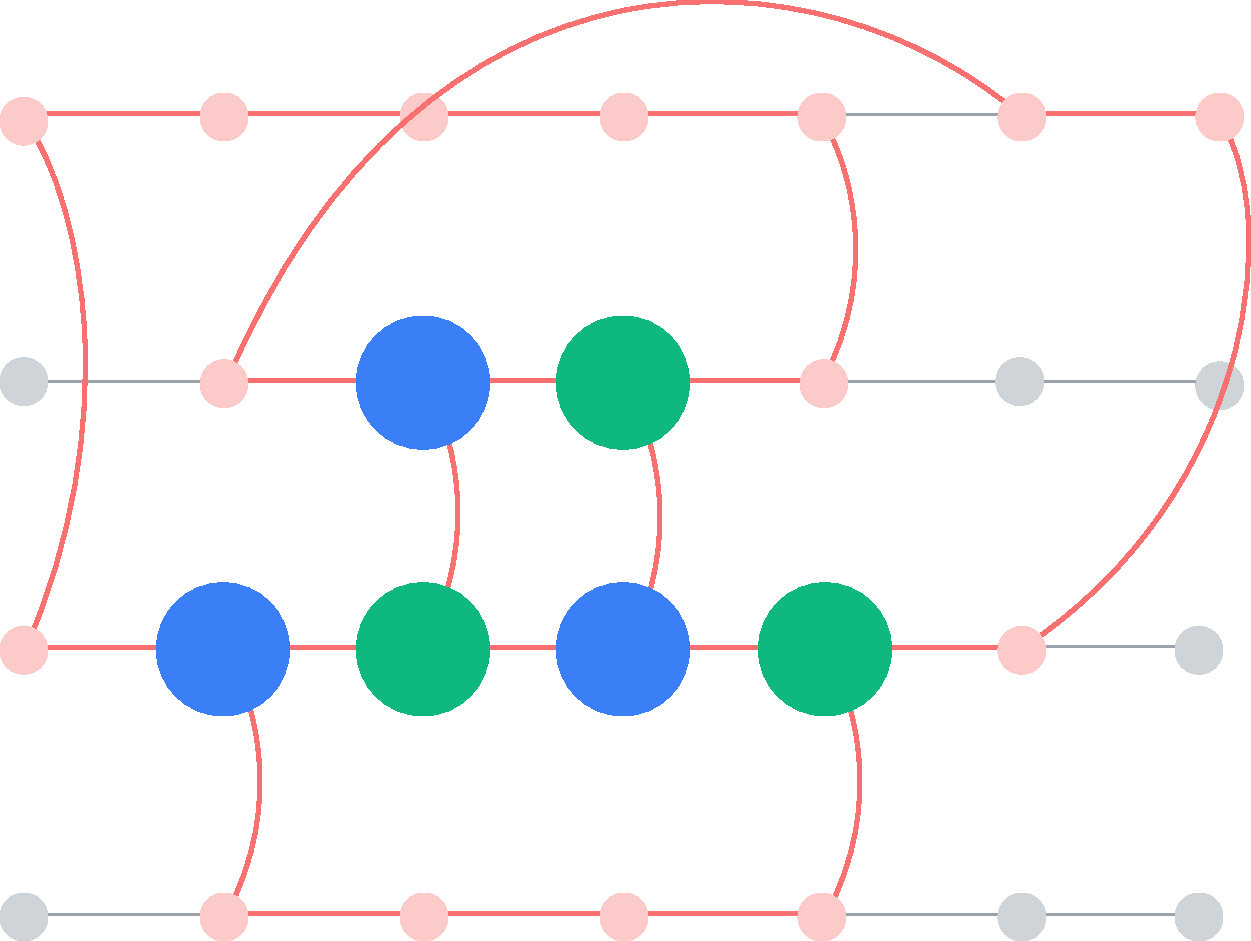
\includegraphics[width=0.9\linewidth]{img/nonplanar.pdf}
  \caption{An example of a valid precursor graph that is not planar due to the presence of a \(K_{3, 3}\) subdivision~\cite{kuratowski1930probleme} (highlighted). Vertices represent amino acid residues, horizontal lines represent peptide bonds, and vertical curved lines represent disulfide bonds. The precursor could be made out of four different interlinked peptides, but it is alsopossible for it to be a single peptide with many intrapeptide disulfide bonds.}\label{fig:nonplanar}
\end{figure}

Let us now say that given a precursor \(R\) a target fragment mass \(f\), we have identified a set \(F\) of connected subgraphs in \(G_R\) with the target mass (or a set of \emph{fragments} for short). Not all of these fragments can occur in real-world measured spectra, even though they do have the correct mass. The number of edges that have at least one vertex in a fragment, but are not themselves in the set of edges of the fragment, represent fragmentation bond cleavages in the original precursor. In HCD, the most common \(b\) and \(y\) fragment ions result from single bond cleavage; so-called internal ions also du occur, but are much more rare. The exact percentage of fragments with 3 or higher number of cleavages is hard to determine in linear peptides, and as far as we know has not been determined in crosslinked peptides, either. However, if they do occur, they will probably be exceedingly rare. The number of cleavages is thus an additional contraint on the fragment matching process.

Apart from these constraints, the simplified versoin ignored some of the inherent complexity of the real mass spectra. First of all, the measured fragment masses are rational numbers, not integers. We also do not need an exact match, but have a tolerance range in which we consider the match to be successful; furthermore, the range is not absolute, but is defined relative to the mass of the generated fragment (in ppm). We also have to take into account the possible modifications of amino acid residues, the possibile occurence of a neutral loss, and the asymetrical nature of disulfide bond cleavage under CID.

All of these add additional complexity to the problem, and make it hard to devise a general well-performing algorithm. What is more, accounting for all of these possibilities creates a big potential of generating false-positive hits due to the great combinatorial power of the matching algorithm. Nevertheless, in the next chapter we describe a general algorithm that attempts to solve the general version of this problem.



% \chapter{Important first chapter}
% \label{chap:refs}

% First chapter usually builds the theoretical background necessary for readers to understand the rest of the thesis. You should summarize and reference a lot of existing literature and research.

% You should use the standard \emph{citations}\todo{Use \textbackslash{}emph command like this, to highlight the first occurrence of an important word or term. Reader will notice it, and hopefully remember the importance.}.

% \begin{description}
% \item[Obtaining bibTeX citation] Go to Google Scholar\footnote{\url{https://scholar.google.com}}\todo{This footnote is an acceptable way to `cite' webpages or URLs. Documents without proper titles, authors and publishers generally do not form citations. For this reason, avoid citations of wikipedia pages.}, find the relevant literature, click the tiny double-quote button below the link, and copy the bibTeX entry.
% \item[Saving the citation] Insert the bibTeX entry to the file \texttt{refs.bib}. On the first line of the entry you should see the short reference name --- from Scholar, it usually looks like \texttt{author2015title} --- you will use that to refer to the citation.
% \item[Using the citation] Use the \verb|\cite| command to typeset the citation number correctly in the text; a long citation description will be automaticaly added to the bibliography at the end of the thesis. Always use a non-breakable space before the citing parenthesis to avoid unacceptable line breaks:
% \begin{Verbatim}
% Trees utilize gravity to invade ye
% noble sires~\cite{newton1666apple}.
% \end{Verbatim}
% \item[Why should I bother with citations at all?] For two main reasons:
% \begin{itemize}
% \item You do not have to explain everything in the thesis; instead you send the reader to refer to details in some other literature. Use citations to simplify the detailed explanations.
% \item If you describe something that already exists without using a citation, the reviewer may think that you \emph{claim} to have invented it. Expectably, he will demand academic correctness, and, from your perspective, being accused of plagiarism is not a good starting point for a successful defense. Use citations to identify the people who invented the ideas that you build upon.
% \end{itemize}
% \item[How many citations should I use?]
% Cite any non-trivial building block or assumption that you use, if it is published in the literature. You do not have to cite trivia, such as the basic definitions taught in the introductory courses.

% The rule of thumb is that you should read, understand and briefly review at least around 4 scientific papers. A thesis that contains less than 3 sound citations will spark doubt in reviewers.
% \end{description}

% There are several main commands for inserting citations, used as follows:
% \begin{itemize}
% \item \citet{knuth1979tex} described a great system for typesetting theses.
% \item We are typesetting this thesis with \LaTeX, which is based on \TeX{} and METAFONT~\cite{knuth1979tex}.
% \item \TeX{} was expanded to \LaTeX{} by \citet{lamport1994latex}, hence the name.
% \item Revered are the authors of these systems!~\cite{knuth1979tex,lamport1994latex}
% \end{itemize}

% \section{Some extra assorted hints before you start writing English}

% Strictly adhere to the English word order rules. The sentences follow a fixed structure with subject followed by a verb and an object (in this order). Exceptions to this rule must be handled specially, and usually separated by commas.


% Mind the rules for placing commas:
% \begin{itemize}
% \item Use the \emph{Oxford comma} before `and' and `or' at the end of a longer, comma-separated list of items. Certainly use it to disambiguate any possible mixtures of conjunctions: \textit{`The car is available in red, red and green, and green versions.'}
% \item Do not use the comma before subordinate clauses that begin with `that' (like this one). English does not use subordinate clauses as often as Slavic languages because the lack of a suitable word inflection method makes them hard to understand. In scientific English, try to avoid them as much as possible. Ask doubtfully whether each `which' and `when' is necessary --- most of these helper conjunctions can be removed by converting the clause to non-subordinate.

% As an usual example, \xxx{\textit{`The sentence, which I wrote, seemed ugly.'}} is perfectly bad; slightly improved by \xxx{\textit{`The sentence that I wrote seemed ugly.'}}, which can be easily reduced to \textit{`The sentence I wrote seemed ugly.'}. A final version with added storytelling value could say \textit{`I wrote a sentence but it seemed ugly.'}
% \item Consider placing extra commas around any parts of the sentence that break the usual word order, especially if they are longer than a single word.
% \end{itemize}

% Do not write long sentences. One sentence should contain exactly one fact. Multiple facts should be grouped in a paragraph to communicate one coherent idea. Paragraphs are grouped in labeled sections for a sole purpose of making the navigation in the thesis easier. Do not use the headings as `names for paragraphs' --- the text should make perfect sense even if all headings are removed. If a section of your text contains one paragraph per heading, you might have wanted to write an explicit list instead.

% Every noun needs a determiner (`a', `the', `my', `some', \dots); the exceptions to this rule, such as non-adjectivized names and indeterminate plural, are relatively scarce. Without a determiner, a noun can be easily mistaken for something completely different, such as an adjective or a verb.

% Consult the books by \citet{glasman2010science} and \citet{sparling1989english} for more useful details.
